\documentclass[11pt]{article}

% ============================================================
% Milestone 2 -- Progress Report
% Project: Lightweight Real-Time Super-Resolution
% ============================================================

\usepackage[margin=1in]{geometry}
\usepackage[T1]{fontenc}
\usepackage[utf8]{inputenc}
\usepackage{amsmath,amssymb}
\usepackage{graphicx}
\usepackage{booktabs}
\usepackage[round]{natbib}
\usepackage{hyperref}
\usepackage{enumitem}
\usepackage{xcolor}
\usepackage{caption}

\hypersetup{
    colorlinks=true,
    linkcolor=blue!50!black,
    citecolor=blue!50!black,
    urlcolor=blue!50!black
}

\setlist[itemize]{noitemsep,topsep=4pt}
\setlist[enumerate]{noitemsep,topsep=4pt}
\graphicspath{{figures/}{./}}

\newcommand{\todo}[1]{\textcolor{red}{\textbf{[TODO: #1]}}}

\title{
    \LARGE Progress Report\\[6pt]
    \large Lightweight Real-Time Super-Resolution\\
    \large for Edge/Laptop Deployment
}

\author{
    Abdelhakeem Osama Abdelhakeem \\ \texttt{2600322}
    \and
    Student B \\ \texttt{}
    \and
    Student C \\ \texttt{}
}

\date{
    Milestone 2 --- November 21, 2026\\{}
    CSE 681 --- Advanced Digital Image and Video Processing
}

\begin{document}
\maketitle

% ============================================================
\begin{abstract}
This project investigates lightweight single-image super-resolution (SISR) for laptop and edge deployment, following the efficiency-oriented evaluation principles of the NTIRE and AIM challenges \citep{ren2025ntire,aim2025}. We implemented EfficientSR, a compact network with depthwise-separable residual blocks, PixelShuffle upsampling and a global bicubic skip connection, and benchmarked it at $\times2$ and $\times4$ against bicubic interpolation and FSRCNN \citep{dong2016fsrcnn} on Set5, Set14, BSD100, Urban100 and Manga109. EfficientSR reaches average Y-channel PSNR of 33.65\,dB ($\times2$) and 27.76\,dB ($\times4$), 2.03\,dB and 1.11\,dB above our FSRCNN baseline. However, it uses more parameters and GMACs than FSRCNN (so the comparison is not yet budget-matched) and is 2.8--3.1 times slower on the CPU. Matched-budget variants and ablations are planned for Milestone 3.
\end{abstract}

% ============================================================
\section{Recap}
\label{sec:recap}
Single-image super-resolution reconstructs a high-resolution (HR) image from a low-resolution (LR) observation. It is important wherever image quality must be improved without better sensors or heavier hardware, but strong models are often too expensive for CPUs and edge devices. The objective of this project is to build and evaluate an efficient $\times2$/$\times4$ SR network under an explicit computational budget of at most 100{,}000 trainable parameters and 10\,GMACs for a $1280\times720$ output (Milestone~1), and to determine whether low GMACs also mean low real-world CPU latency.

Training and validation use DIV2K \citep{agustsson2017div2k}; evaluation uses Set5, Set14, BSD100, Urban100 and Manga109. Bicubic interpolation and FSRCNN \citep{dong2016fsrcnn} are the reference methods (ESPCN \citep{shi2016espcn} is planned). The metrics are Y-channel PSNR and SSIM, the number of parameters, GMACs for a $1280\times720$ output, and measured CPU latency. The project scope is unchanged since Milestone~1; this milestone completes both the $\times2$ and the $\times4$ comparison.

% ============================================================
\section{Implementation Status}
\label{sec:status}
The training and evaluation pipeline is implemented in Python/PyTorch and runs on Windows. Training used an NVIDIA GeForce RTX 3060 Laptop GPU (6\,GB); CPU measurements used an Intel Core i5-11400H (6 cores, 12 threads) with 16\,GB RAM. The implementation supports:
\begin{itemize}
    \item training at $\times2$ and $\times4$ with per-epoch validation, atomic checkpoints and resume;
    \item benchmarking on all five test sets with one command;
    \item Y-channel PSNR/SSIM, parameter counts, GMACs and CPU latency;
    \item generation of sample images for visual comparison.
\end{itemize}

\paragraph{Training setup.} LR images are created on the fly with PIL bicubic resampling from random scale-aligned $96\times96$ HR patches (about 20 per DIV2K image per epoch) with flips and $90^\circ$ rotations. All models use the $L_1$ loss, Adam (initial learning rate $10^{-3}$, halved every $\lfloor E/3\rfloor$ epochs for $E$ epochs), batch size 32, seed 0, and validation on the first 50 DIV2K validation images.

\paragraph{Evaluation protocol.} PSNR and SSIM are computed on the Y channel (ITU-R BT.601) after rounding outputs to 8 bit and shaving a border of \texttt{scale} pixels; ``Avg.'' is the unweighted mean over the five test sets. GMACs count learned convolution and transposed-convolution layers for a $1280\times720$ output (FLOPs $\approx2\times$MACs; the bicubic skip is not counted). CPU latency is the median of 20 runs after warm-up with 4 threads, end to end for a $1280\times720$ output.
The code and results are available at \url{https://github.com/kimoz1251h/Lightweight-sr}.

\subsection{Baseline Reproduction}
Bicubic interpolation and FSRCNN ($d=56$, $s=12$, $m=4$) were evaluated with the same pipeline. FSRCNN was trained at $\times2$ (65 epochs) and at $\times4$ (70 epochs). Results are in Tables~\ref{tab:x2_results}--\ref{tab:x4_datasets}.

Our FSRCNN scores are lower than those published in the original paper \citep{dong2016fsrcnn}:
for $\times2$ we obtain 35.15\,dB on Set5 and 31.53\,dB on Set14, compared with 37.00\,dB and
32.63\,dB reported there (gaps of about 1.9\,dB and 1.1\,dB). Several differences between the
setups explain this. The original model processes a single channel and has about 12k parameters,
whereas ours takes RGB input and has 24,683 parameters; it was trained on the 91-image and
General-100 sets, whereas we train on DIV2K only with a short schedule. In addition, LR images are
generated with PIL rather than MATLAB \texttt{imresize}, and we shave \texttt{scale} border pixels
(as noted in Milestone~1). Absolute values should therefore be compared only within this report,
where all methods share exactly the same protocol.

\subsection{Proposed Method: EfficientSR}
EfficientSR consists of a $3\times3$ head convolution, $N$ residual blocks (depthwise $3\times3$, pointwise $1\times1$, PReLU, pointwise $1\times1$, skip connection) with a long skip from the head, a $3\times3$ tail convolution producing $3s^2$ channels, PixelShuffle upsampling, and an optional global bicubic skip. The trained configuration uses $C=48$ channels and $N=6$ blocks (C48B6): $\times2$ for 65 epochs and $\times4$ for 70 epochs. Both models are inside the project budget (Table~\ref{tab:x2_results}: 37{,}932 parameters, 8.460 GMACs at $\times2$; Table~\ref{tab:x4_results}: 53{,}520 parameters, 3.011 GMACs at $\times4$). The checkpoints were used for the benchmark below. ESPCN and the no-skip ablation are implemented in the code but not yet trained.

% ============================================================
\section{Preliminary Results}
\label{sec:results}
All numbers use the protocol above. Average values are means over Set5, Set14, BSD100, Urban100 and Manga109. The CPU times below were measured on an otherwise idle machine and replace the provisional values given in Milestone~1 (which were taken while training was running).

\subsection{Quantitative Results: $\times2$}
\begin{table}[htbp]
\centering
\caption{Quantitative comparison for $\times2$ super-resolution (CPU: i5-11400H, 4 threads, $1280\times720$ output).}
\label{tab:x2_results}
\small
\begin{tabular}{@{}lccccc@{}}
\toprule
\textbf{Method} & \textbf{Avg. PSNR} & \textbf{Avg. SSIM} & \textbf{Params} & \textbf{GMACs} & \textbf{CPU (ms)} \\
\midrule
Bicubic & 30.52 & 0.8883 & 0 & 0.000 & 15 \\
FSRCNN & 31.62 & 0.9082 & 24,683 & 5.607 & 159 \\
\textbf{EfficientSR} & \textbf{33.65} & \textbf{0.9273} & 37,932 & 8.460 & 448 \\
\bottomrule
\end{tabular}
\end{table}

EfficientSR improves the average PSNR by 2.03\,dB and SSIM by 0.0191 over FSRCNN, at the cost of 50.9\% more GMACs, 53.7\% more parameters, and a CPU latency that rises from 159\,ms to 448\,ms.

\subsection{Quantitative Results: $\times4$}
\begin{table}[htbp]
\centering
\caption{Quantitative comparison for $\times4$ super-resolution (same setup).}
\label{tab:x4_results}
\small
\begin{tabular}{@{}lccccc@{}}
\toprule
\textbf{Method} & \textbf{Avg. PSNR} & \textbf{Avg. SSIM} & \textbf{Params} & \textbf{GMACs} & \textbf{CPU (ms)} \\
\midrule
Bicubic & 25.84 & 0.7293 & 0 & 0.000 & 15 \\
FSRCNN & 26.65 & 0.7592 & 24,683 & 1.402 & 40 \\
\textbf{EfficientSR} & \textbf{27.76} & \textbf{0.7927} & 53,520 & 3.011 & 122 \\
\bottomrule
\end{tabular}
\end{table}

At $\times4$ EfficientSR improves the average PSNR by 1.11\,dB and SSIM by 0.0335, with 114.8\% more GMACs, 116.8\% more parameters and a CPU latency that rises from 40\,ms to 122\,ms.

\subsection{Dataset-Level Results}
\begin{table}[htbp]
\centering
\caption{PSNR (dB) / SSIM for $\times2$ super-resolution.}
\label{tab:x2_datasets}
\small
\begin{tabular}{@{}lccc@{}}
\toprule
\textbf{Dataset} & \textbf{Bicubic} & \textbf{FSRCNN} & \textbf{EfficientSR} \\
\midrule
BSD100   & 29.74 / 0.8495 & 30.63 / 0.8789 & \textbf{31.59 / 0.8920} \\
Set14    & 30.56 / 0.8750 & 31.53 / 0.8971 & \textbf{32.79 / 0.9103} \\
Set5     & 33.97 / 0.9330 & 35.15 / 0.9445 & \textbf{37.16 / 0.9573} \\
Manga109 & 31.25 / 0.9384 & 32.78 / 0.9499 & \textbf{36.57 / 0.9715} \\
Urban100 & 27.07 / 0.8456 & 28.01 / 0.8705 & \textbf{30.14 / 0.9055} \\
\bottomrule
\end{tabular}
\end{table}

\begin{table}[htbp]
\centering
\caption{PSNR (dB) / SSIM for $\times4$ super-resolution.}
\label{tab:x4_datasets}
\small
\begin{tabular}{@{}lccc@{}}
\toprule
\textbf{Dataset} & \textbf{Bicubic} & \textbf{FSRCNN} & \textbf{EfficientSR} \\
\midrule
BSD100   & 26.05 / 0.6721 & 26.57 / 0.7008 & \textbf{27.07 / 0.7185} \\
Set14    & 26.22 / 0.7088 & 26.95 / 0.7383 & \textbf{27.83 / 0.7626} \\
Set5     & 28.63 / 0.8137 & 29.72 / 0.8428 & \textbf{30.92 / 0.8744} \\
Manga109 & 25.07 / 0.7904 & 26.13 / 0.8187 & \textbf{28.23 / 0.8716} \\
Urban100 & 23.24 / 0.6615 & 23.87 / 0.6954 & \textbf{24.75 / 0.7365} \\
\bottomrule
\end{tabular}
\end{table}

EfficientSR obtains the highest PSNR and SSIM of the three methods on all five datasets at both scales. The gains are largest on Manga109 and Urban100 (up to 3.8\,dB and 2.1\,dB over FSRCNN at $\times2$), which contain strong edges and repeated structures.

\subsection{Quality versus Computational Cost}
The quality gain of EfficientSR is paid for in computation. At $\times2$ it needs 1.51 times the GMACs of FSRCNN (8.460 vs.\ 5.607) but is 2.82 times slower on the CPU (448 vs.\ 159\,ms); at $\times4$ it needs 2.15 times the GMACs (3.011 vs.\ 1.402) and is 3.05 times slower (122 vs.\ 40\,ms). In both cases the measured latency grows faster than the GMAC count, which is consistent with our hypothesis that depthwise-separable blocks cost more real CPU time than their GMACs suggest. This is not yet proven, because EfficientSR and FSRCNN also differ in depth and in their upsampling layers; the planned comparison with a standard-convolution variant at equal GMACs (Section~\ref{sec:next}) will test it.

In absolute terms, EfficientSR at $\times2$ needs 448\,ms per $1280\times720$ output frame (about 2 frames per second) and FSRCNN 159\,ms (about 6 frames per second), so neither is real time for $\times2$ video on this CPU, whereas bicubic takes 15\,ms. At $\times4$ the models are faster because most computation happens on a much smaller LR input (EfficientSR 122\,ms, about 8 frames per second).

Importantly, EfficientSR is inside the project budget but \emph{not} matched to FSRCNN: it has more parameters and GMACs, so part of its quality advantage may simply come from its larger size or from the bicubic global skip. A fair attribution requires the matched-budget variants and the no-skip ablation planned for Milestone~3. The GMAC counts include only learned convolutions (the bicubic skip is not counted), while the latency includes the whole forward pass.

\subsection{Qualitative Comparison}
Figures~\ref{fig:visual_x2} and~\ref{fig:visual_x4} show the same cropped region of BSD100 image 101085 for ground truth, bicubic, FSRCNN and EfficientSR.

\begin{figure}[htbp]
\centering
\IfFileExists{final_comparison_x2.png}{%
    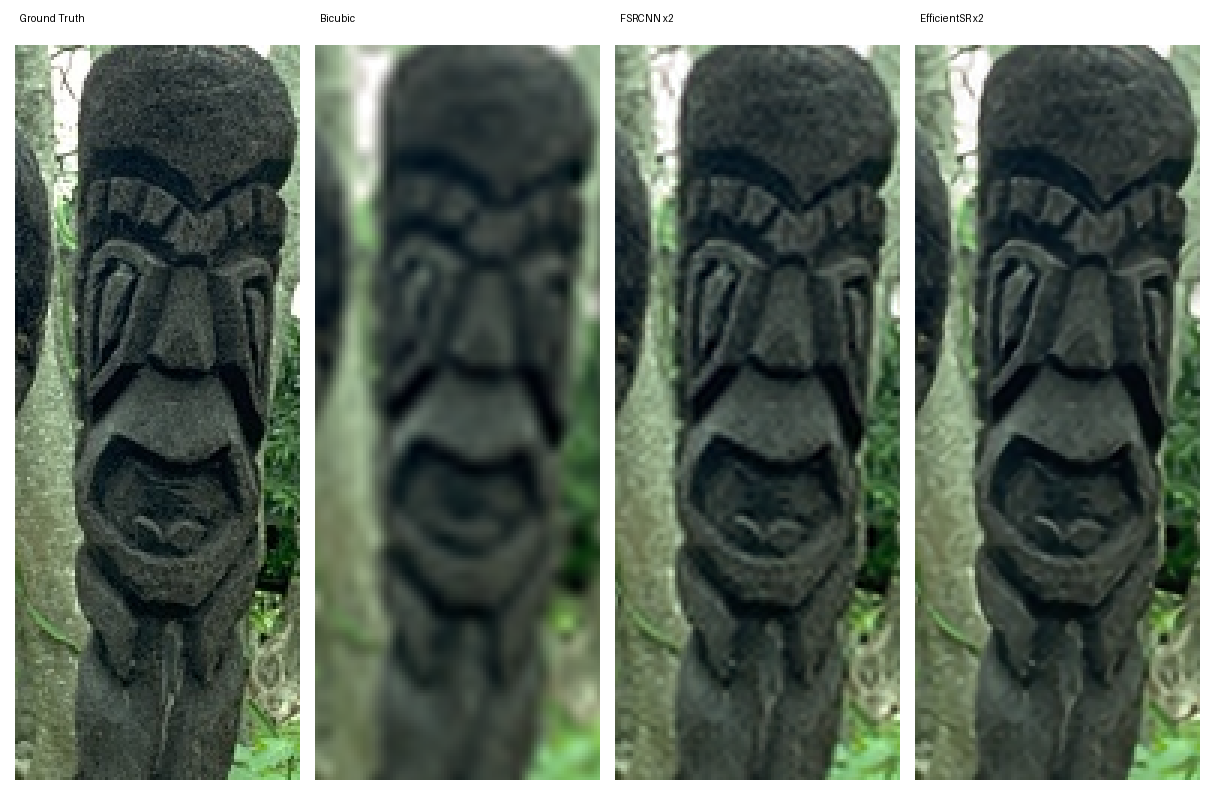
\includegraphics[width=\textwidth]{final_comparison_x2.png}%
}{%
    \fbox{\parbox{0.8\textwidth}{\centering Place final\_comparison\_x2.png in the project directory.}}%
}
\caption{$\times2$ comparison (BSD100, image 101085, cropped). Left to right: ground truth, bicubic, FSRCNN, EfficientSR.}
\label{fig:visual_x2}
\end{figure}

At $\times2$ bicubic is clearly blurred. FSRCNN restores the carved facial structure and EfficientSR gives a similar but slightly cleaner reconstruction of the stone texture. Both learned models are smoother than the ground truth, which keeps its fine grain.

\begin{figure}[htbp]
\centering
\IfFileExists{final_comparison_x4.png}{%
    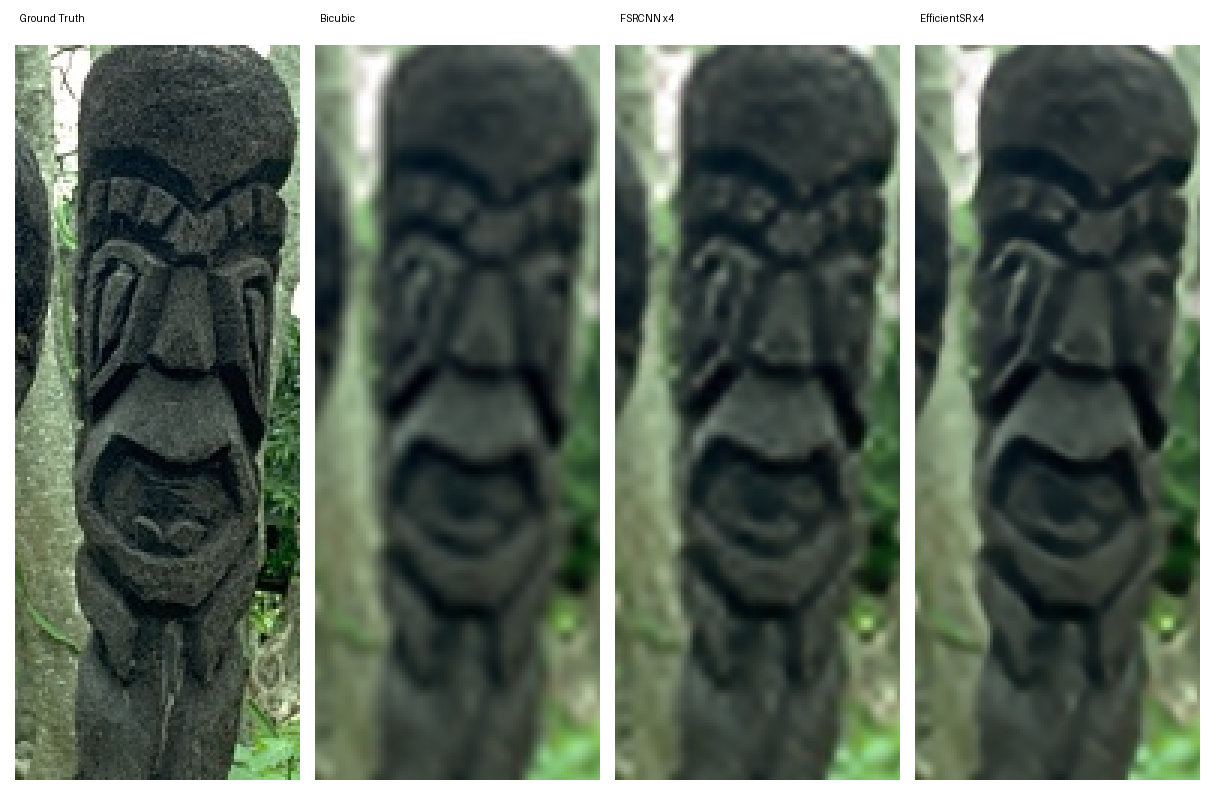
\includegraphics[width=\textwidth]{final_comparison_x4.png}%
}{%
    \fbox{\parbox{0.8\textwidth}{\centering Place final\_comparison\_x4.png in the project directory.}}%
}
\caption{$\times4$ comparison (same image and crop as Figure~\ref{fig:visual_x2}).}
\label{fig:visual_x4}
\end{figure}

At $\times4$ all methods lose much of the fine detail. EfficientSR preserves the overall facial structure, but its visual advantage over FSRCNN is small in this example, even though its average PSNR is 1.11\,dB higher. The qualitative observations should be read together with the numbers over all five datasets.

% ============================================================
\section{Challenges \& Deviations from the M1 Plan}
\label{sec:challenges}
\begin{itemize}
    \item \textbf{GPU failure during training.} During EfficientSR $\times4$ training a CUDA ``unspecified launch failure'' occurred. Training was resumed from the last saved checkpoint after restarting the computer, and the run was completed.
    \item \textbf{Slow training.} One epoch took about 9--10 minutes in our measurements while the GPU was only 13--18\% utilized, so the data loader (decoding large DIV2K images) is the bottleneck. We will use cached crops or more data-loading workers for the ablation runs.
    \item \textbf{Quality--cost trade-off.} EfficientSR is more accurate than FSRCNN but also larger and slower; the comparison is not budget-matched (Section~\ref{sec:results}).
    \item \textbf{CPU latency.} The M1 timings were taken while training was running; they were re-measured on an idle machine (Tables~\ref{tab:x2_results} and~\ref{tab:x4_results}), and these final numbers replace the provisional ones.
    \item \textbf{Visual versus quantitative evaluation.} Higher average PSNR/SSIM does not always give an equally visible improvement in a single image, so both are reported.
    \item \textbf{Baseline strength.} Our FSRCNN is weaker than the published model (Section~\ref{sec:status}), so results are valid only within our shared protocol.
\end{itemize}
The project direction is unchanged; we completed both $\times2$ and $\times4$ comparisons, which the M1 MVP required.

% ============================================================
\section{Updated Work Breakdown \& MVP Status}
\label{sec:workbreakdown}
Status of the Milestone~1 minimum viable deliverable:
\begin{itemize}
    \item[$\checkmark$] A complete $\times2$ super-resolution pipeline.
    \item[$\checkmark$] A complete $\times4$ experiment with a matching FSRCNN $\times4$ baseline.
    \item[$\checkmark$] Bicubic and trained FSRCNN baselines on the test sets.
    \item[$\checkmark$] Trained EfficientSR configurations (C48B6, $\times2$ and $\times4$).
    \item[$\checkmark$] Evaluation on all five benchmark datasets.
    \item[$\checkmark$] PSNR/SSIM, parameter, GMAC and CPU-time measurements.
    \item[$\circ$] A recorded demo ($\le5$ minutes): not yet done, planned for Milestone~3.
\end{itemize}
The core experimental part of the MVP has therefore been reached; the demo, the ablations and the final documentation remain.

\begin{table}[htbp]
\centering
\caption{Updated milestone task allocation.}
\label{tab:tasks}
\small
\begin{tabular}{@{}p{0.14\linewidth}p{0.27\linewidth}p{0.27\linewidth}p{0.27\linewidth}@{}}
\toprule
\textbf{Milestone} & \textbf{Student A --- Data \& Baseline} & \textbf{Student B --- Model} & \textbf{Student C --- Evaluation} \\
\midrule
M2 --- completed &
Data pipeline and test sets; FSRCNN training ($\times2$, $\times4$) and baseline benchmarks &
EfficientSR implementation; training at $\times2$ and $\times4$ &
Metrics, GMAC and CPU-timing code; benchmark tables; qualitative comparisons \\
M3 --- planned &
Final FSRCNN numbers; ESPCN baseline; cached crops for faster training &
Matched-budget variants; width/depth and bicubic-skip ablations; standard-convolution variant &
Final PSNR/SSIM/runtime tables and plots; demo; final report \\
\bottomrule
\end{tabular}
\end{table}

% ============================================================
\section{Next Steps}
\label{sec:next}
\begin{enumerate}
    \item \textbf{Matched-budget comparison:} train EfficientSR variants with parameters matched to FSRCNN and with GMACs matched to FSRCNN, so that the quality difference can be attributed to the architecture.
    \item \textbf{Ablations:} width/depth study (parameter/GMAC budget) and the no-skip variant (\texttt{--no-skip}) to measure the contribution of the bicubic skip; a standard-convolution variant at equal GMACs to test the depthwise-latency hypothesis.
    \item \textbf{ESPCN baseline} at $\times2$ and $\times4$.
    \item \textbf{CPU optimization:} investigate whether latency can be reduced (for example thread count, channels-last memory format or operator fusion) while keeping quality.
    \item \textbf{Demo:} a script that loads a checkpoint and enlarges a user-provided image on the CPU, plus the recorded demo (at most 5 minutes).
    \item \textbf{Final report:} full tables and plots (PSNR/SSIM versus CPU time), failure cases, limitations, training configurations and reproducibility information.
\end{enumerate}

% ============================================================
\section{Conclusion}
\label{sec:conclusion}
EfficientSR improves reconstruction quality over our FSRCNN baseline on all five test sets at both scales (average PSNR 33.65\,dB and 27.76\,dB), and both models stay within the project budget. The improvement is accompanied by higher parameter counts, GMACs and, disproportionately, CPU latency, and the comparison is not yet budget-matched. Milestone~3 will therefore concentrate on matched-budget variants, ablations, optimization and the demo, to answer whether a lightweight model can be both accurate and genuinely fast on a CPU.

\paragraph{AI-use disclosure.} AI assistance (ChatGPT and Claude) was used for LaTeX drafting, clarification of technical concepts, and code debugging. All technical decisions, experiments, results, and final content were reviewed and verified by the team.

\bibliographystyle{unsrtnat}
\bibliography{references}

\end{document}